\documentclass[thesismargins, english, thesislinespacing, onelinechapterstyle, upjsfrontpage]{rnthesis}
\usepackage[english]{babel}
\usepackage[T1]{fontenc}
\usepackage[utf8]{inputenc}
\usepackage{lmodern}

\usepackage{rnt-pic}
\usepackage{rnt-thm}

\usepackage{pdfpages} % inserting pdf pages

\usepackage[hyphens]{url} % format and linebreak of URLs

\usepackage{tikz}
\usetikzlibrary{datavisualization}
\usetikzlibrary{datavisualization.formats.functions}

\usepackage{xparse}
% Rotation: \rot[<angle>][<width>]{<stuff>}
\NewDocumentCommand{\rot}{O{60} O{1em} m}{\makebox[#2][l]{\rotatebox{#1}{#3}}}%

\title{Replacing handwritten signatures with open electronic signature software}
\author{Jakub Ďuraš}
\iffalse % Not part of the version for ŠVK
\typprace{bachelor's}
\fi
\inytypprace{Student Scientific Conference}
\rok{2020}
\odbor{Applied Informatics}
\miesto{Košice}
\veduci{RNDr. Viliam Kačala}
\pracovisko{Institute of Computer Science}
\iffalse % Not part of the version for ŠVK
\podakovanie{
  I would like to thank my supervisor Viliam Kačala for his continuous feedback and patience with my question.

  I would also like to acknowledge help received from Pavol Sokol and Laura Rózenfeldová on legal questions, and access to various resources from Gabriel Semanišin.

  Finally, I would like to thank my family and friends who contributed in various ways to my thesis.
}
\fi

\iffalse % Not part of the version for ŠVK
\pdfzadanie{zadanie.pdf}
\fi


\abstract{
With the recent changes in the legal status of electronic signatures in the world, there is an opportunity to expand the use of electronic signatures as an alternative to handwritten signatures outside the usual areas.
Electronic signatures are becoming increasingly important in the age of electronic communication when handwritten signatures are unpractical due to the need to print, personally exchange, or send signed documents.
We devote our attention to the exploration of legal preconditions relevant for the EU, technological preconditions, review of the existing software, and proposal of our own software platform.
The result is open, user-friendly software for Windows, Mac OS X, and Linux.
Using the application, it is possible, following the eIDAS Regulation, to sign and verify the signature of any document with the legal effect of an attested signature.
Our solution supports ID cards of the Slovak Republic with the eID chip without any modifications or settings, which enables easy use outside the usual use in web applications of the state.
The application is not tied only to the Slovak eID but is ready for further use with various devices in different countries and as a platform for other types of signatures.
Another part is a website that, in addition to the possibility of downloading software and brief documentation, provides general information about electronic signatures so that the project is as accessible to the public as possible.
We concentrate on simple extensibility of the program via language translations, documentation, functionality, and general information.
}

\keywords{electronic signature, electronic seal, qualified, open-source, XAdES, PAdES, CAdES, desktop software}

\abstrakt{
So zmenami v právnom statuse elektronických podpisov vo svete sa vytvára príležitosť rozšíriť elektronické podpisovanie ako náhradu pre vlastnoručné podpisy mimo obvyklých oblastí.
Elektronické podpisy sú dôležité čoraz viac v dobe elektronickej komunikácie kedy sú vlastnoručné podpisy nepraktické z dôvodu nutnosti tlače, osobného kontaktu alebo zasielania podpísaných dokumentov.
V práci sa venujeme právnym predpokladom relevantným pre EÚ, technologickým predpokladom, prehľadu v súčasnosti dostupného softvéru a návrhu vlastnej softvérovej platformy.
Výsledkom je otvorený, používateľsky prívetivý softvér pre platformy Windows, Mac OS X a Linux.
Pomocou aplikácie je možné, v súlade s nariadením eIDAS, podpísať a overiť podpis ľubovoľného dokumentu, ktorý má rovnaký právny účinok ako osvedčený podpis.
Naše riešenie podporuje občianske preukazy Slovenskej Republiky s čipom eID bez akýchkoľvek úprav alebo nastavení, čím sa umožní ich jednoduché využitie mimo obvyklého použitia vo webových aplikáciách štátu.
Aplikácia nie je viazaná iba na slovenské eID, ale je pripravená na ďalšie použitie s rôznymi zariadeniami v rôznych štátoch a ako platforma pre iné druhy podpisov.
Súčasťou je aj webová stránka, ktorá okrem možnosti stiahnutia softvéru a stručnej dokumentácie poskytuje všeobecné informácie o elektronických podpisoch aby bol projekt čo najviac prístupný verejnosti.
Dôraz kladieme na jednoduchú rozšíriteľnosť programu vo forme jazykových prekladov, dokumentácie, funkcionality a všeobecných informácií.
}

\klucoveslova{elektronický podpis, elektronická pečať, kvalifikovaný, open-source, XAdES, PAdES, CAdES, počítačový softvér}

\bibliographystyle{alpha}

\begin{document}
\maketitle

\newpage

\tableofcontents
\iffalse % Not part of the version for ŠVK
\listoffigures
\listoftables
\fi

\uvod

Electronic signatures have been around for a while.
Their practical usability, however, is influenced by their legal status and available infrastructure.
With the recent changes in the relevant law around the world and the European Union specifically, they see increased adoption.

While, specifically in the European Union, they seem to be relatively extensively used in communication with the government, they do not seem to be widely adopted in an exchange between individuals or smaller organizations.
The problem is handwritten signatures are often unpractical for electronic communication due to the need to print, personally exchange, or send signed documents.

Our goal is to explore an accessible way to use electronic signatures.
In the beginning, we go over the preconditions that make it a viable alternative to the handwritten signatures.
We cover the legal preconditions relevant for the European Union and Slovakia in particular.
Also, we explain technical preconditions focusing on the cryptographic concepts like asymmetric cryptography, timestamping, hashing, and standards that comply with the law within the European Union.
Secondly, we do a review of the existing software.
We go quickly over several applications that are meant for basic use.
We compare them using several criteria to find out the strengths and weaknesses of the current implementations and identify a potential space for improvements.
Finally, we devote our attention to our own implementation.
We explain the proposed desktop software and go into details on software engineering aspects.
Specifically, modularity, architecture, usability, localization, testing, and automation.
In the end, we compare it with the existing software and identify possible future improvements.
Another result we focus on is a supporting website and how it helps with the use of the software.
All in a way open for extensibility by the community.

\chapter{Preconditions and theory}

There are several preconditions that allow us to consider electronic signatures as an alternative.
Firstly, the current state of the law and recent changes relating to the use of electronic signatures, secondly, well-established concepts in cryptography like \pojem{asymmetric cryptography} or \pojem{hashing}, and lastly, expertise from the field of software engineering - design, implementation, and maintenance of computer software.
We will concetrate on the first two in relation to the electronic signatures, and, where applicable, open-source desktop computer software.

\iffalse % Not part of the version for ŠVK
TODO: Think about adding section on handwritten signatures
\fi

\section{Law}

We are considering law applicable locally in the Slovak Republic (SR).
Its law is greatly influenced by the European Union (EU), being its member since 2004, and by the rest of the world.
We can assume this is at least partially applicable outside of the SR as well.

\subsection{Signatures}

Signatures are an essential part of the written legally binding documents like contracts.
They are permanently affixed to the document and are supposed to uniquely identify the person and its deliberate, informed consent.
As can be seen in the Slovak Civil Code, § 40, a written legal act is valid if signed by the acting person \cite{civilcode}.
Our law often explicitly requires signatures and further clarifies their expected use.
For example, when selling an enterprise, looking at the Commercial Code, § 476, the contract requires written form and attested signatures of the seller and the buyer \cite{commercialcode}.

Signature is considered an "attested signature"\footnote{Translation from "osvedčený podpis" as used in the Slovak law.} if it is verified by an authorized third party.
This process is referred to as legalization in Notary Law, § 56, and its purpose is to attest information that could form the basis for the exercise of rights or which could cause legal consequences \cite{notarylaw}.

With regards to electronic signatures, law within the EU used to differ, with the law applicable in the SR being now-repealed \pojem{Act No. 215/2002 Coll.}. This situation changed with the EU Regulation eIDAS.

\subsection{EU Regulation eIDAS} \label{eidas}

With intention to stimulate digital growth by building trust, the EU established regulation on electronic identification and trust services for electronic transactions in the internal market (eIDAS).
It applies from 1st of July 2016, replaces local law, and regulates, among other things, electronic signatures and its more specific variants.

\obrazok{./figures/electronic-advanced-qualified}{The relation between electronic, advanced, and qualified signatures.}{signature-comparison}

In general, electronic signature can be represented in different ways (e.g. as an image, text or other data attached to the document) and they \textbf{can not be denied in legal proceedings} just because they are in the electronic form \cite{eidas}.

\pojem{Advanced electronic signatures} are a subset of electronic signatures that have to \textbf{uniquely link and identify} the signature author, be created in a way that is \textbf{possible only by them} and any \textbf{changes to the signed document have to be detectable} \cite{eidas}.
From the technical point of view, standards \pojem{PAdES}, \pojem{XAdES}, and \pojem{CAdES} specified by the European Telecommunications Standards Institute (ETSI) comply with these requirements. We explain why this is the case in Section \ref{cryptography}.

\pojem{Qualified electronic signatures} (QES) are a subset of \pojem{advanced electronic signatures} with more specific requirements that can be found in annex 1 of the eIDAS regulation\footnote{Available at https://eur-lex.europa.eu/legal-content/EN/TXT/HTML/?uri=CELEX:32014R0910\#d1e32-111-1.}.
In more practical terms, such \pojem{advanced electronic signatures} are created with a qualified device using a qualified certificate and a qualified trust service.
Qualified, in this case, means authorized for such use by the legal authorities.
These devices, \pojem{certificates}, and trust services are explicitly listed by the EU. In many cases indirectly by listing the organization (and its items) from a specific country.

Furthermore, a qualified electronic signature has the legal effect of a handwritten signature \cite{eidas} and attested handwritten signatures in the SR.

Mentioned terminology is used when considering a natural person. Legal entities are able to use \pojem{electronic seals}, which are, from the technical point of view and for our purposes, identical.

Overall, electronic signatures are supposed to be, within the EU, interoperable and transparent alternative to handwritten signatures.

\subsection{Software copyright} \label{copyright}

Computer programs and associated materials are historically protected under copyright as literary works, and protected authors should be able to authorize or prohibit certain acts \cite{eeccopyright}.

Such right can be exercised to license the software under either \pojem{proprietary} or \pojem{open-source} license.
\pojem{Proprietary} meaning under the exclusive legal right of the author, typically also \textbf{confidential and distributed as a paid product}.
\pojem{Open-source} meaning having its source code \textbf{freely available}, typically also \textbf{distributed for free} and without any liability (the software is provided "as is").

Motivation to license the software under an \pojem{open-source} license can differ, and so do such licenses.
While a \pojem{proprietary} license is usually made specifically for that entity and its interests, \pojem{open-source} licenses tend to be reused between different authors.
This means that consumers of the software can quickly recognize their rights and responsibilities if they decide to use, modify, or distribute the software.
In general, we can classify the \pojem{open-source} licenses into two categories: \pojem{permissive} and \pojem{copyleft}.

\pojem{Copyleft} license, in general, requires the user to publish the modified work under the compatible (free) license.
As a result, it forces them to extend the rights they have received onto others and, in turn, somehow hinder usability in software licensed under a different license.
A popular example of such license is the GNU General Public License(GPL) and its derivatives like GNU Lesser GPL (LGPL) or GNU Affero GPL (AGPL).

\pojem{Permissive} licenses, on the other hand, do not have such a requirement in place and are more suitable for potential commercialization.
They typically allow commercial use, modifications, distribution or sublicensing as long as the author is not held liable, and the original copyright and license are distributed with the software.
Often used permissive licenses are MIT License, Apache License, or BSD License.

It is not uncommon to see \pojem{hybrid licensing} - licensing under more than one license, with one being typically \pojem{open-source} and one \pojem{proprietary}.
In this scenario, users can choose which license they want to use based on their needs.

\obrazok{./figures/license-comparison}{Classification and comparison of software licensing models.}{license-comparison}

As we have already mentioned, software licenses can influence whether and how it can be used as a part of different software.
Both when we are the ones using someone else's software and when someone else is using our software.
Generally speaking, the more open the license is, the higher the probability it will not prevent adoption for legal reasons.
Various possible combinations can be seen in Figure \ref{fig:license-compatibility}, where greyed out options mean such combination is not possible unless a separate licensing agreement is reached with the copyright owner.

\obrazok{./figures/license-compatibility}{Schematic representation of license directionality. \osoba{Morin 2012} \cite{licensing}}{license-compatibility}

\section{Cryptography} \label{cryptography}

Previously mentioned standards \pojem{PAdES}, \pojem{XAdES}, and \pojem{CAdES} define how \pojem{asymmetric cryptography}, \pojem{hashing}, or \pojem{timestamping} should be used to comply with the standards.
We go over a these topics and why they are able to satisfy the requirements for QES mentioned in the Section \ref{eidas}.

\subsection{Asymmetric cryptography}

There are several issues that make symmetric encryption unsuitable.
Let us imagine we are creating a key for each pair of users in our network - imaginary country Isle of Alices and Bobs - for symmetric encryption and decryption of documents shared between each Alice and Bob.

\textbf{Secure distribution of keys} seems to be feasible when we are adding a new user to our network.
We require each user to personally come and pick up a physical device that contains pre-generated keys.
Changes made after that, however, would mean we either need to require a periodic personal visit to update the saved keys or transmission of these keys over some medium, which can be potentially unsafe.
Any new members of the network are unable to participate until other Alices and Bobs get their updates.

Even if we think we have established a reasonably secure way to do that and we are willing to wait, we realize the \textbf{number of keys} is quickly increasing with each new member. With \textit{n} users, the number of keys is

$$\frac{n \cdot (n - 1)}{2}$$

which means that even our little imaginary country with a population of only 70 000 requires roughly 2.5 billion keys. However, since our signature system needs to be portable, we will need to count also with a population of other countries, and so the number of keys grows very quickly.

\iffalse % Not part of the version for ŠVK
\begin{figure}[!htb]
  \centering

  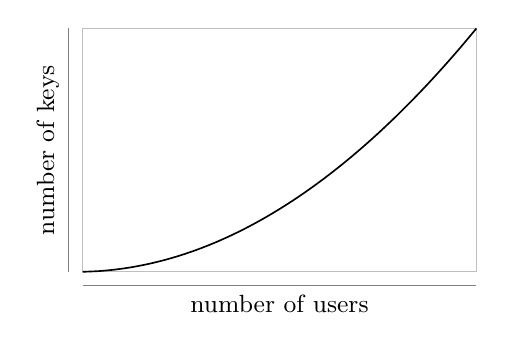
\begin{tikzpicture}
    \datavisualization [scientific axes=clean, visualize as smooth line, all axes={ticks={major={at={}}}}, y axis={label={number of keys}}, x axis={label={number of users}}]
    data [format=function] {
      var x : interval [2:125];
      func y = \value x*\value x;
    };
  \end{tikzpicture}

  \centerline{\parbox{13cm}{\sl \caption{Cubic growth of the number of keys.}}}
\end{figure}
\fi

\textbf{Either party can also lie} about not signing the document.
Since both have the key that can be used for encryption, they can sign any document on behalf of the other party, and there is no way to disprove it if we look at it as a third party.

These issues can be addressed with \pojem{asymmetric cryptography}.
In general, we assign \textbf{a pair of keys} to each person, one of them used for encryption, known as a \pojem{public key}, another used for decryption, known as a \pojem{private key}.
One party can encrypt, and the other is the only one that can decrypt.

\pojem{Digital signatures} are specific \pojem{asymmetric cryptography} algorithms.
The signer is the only one who possesses the \pojem{private key} used for signing, and others can use the \pojem{public key} for signature verification.
We \textbf{sign} the document, including the other parties' signature.

\iffalse % Not part of the version for ŠVK
\obrazok{./figures/digital-signature-scheme}{Principle of digital signatures which involves signing and verifying a message (Paar 2009). TODO: I don't have rights to this image!!!}{pubkey-scheme}
\fi

Practical, widely used implementation of this idea is the \pojem{RSA} signature scheme that relies on the integer factorization problem (difficulty of factoring a product of two large primes) published in 1978 \cite{rsa}.

In Slovakia, the private key is usually handed over to the user personally, saved on the ID card. This ID card (used together with a card reader) provides an API for safe access, management, and cryptoprocessing.
Such a device is in general called a \pojem{Hardware Security Module} (HSM), and the API relevant for this thesis is \pojem{PKCS \#11} \footnote{PKCS \#11 specification available at \url{http://docs.oasis-open.org/pkcs11/pkcs11-base/v2.40/os/pkcs11-base-v2.40-os.html}.}.

We are left with the \textbf{problem of public key distribution} - even though \pojem{public-key schemes} do not require a \textit{secure channel}, they require \textit{authenticated channels} for the distribution of the public keys \cite{cryptotxtbook}.

A common solution is the use of \pojem{certificates}. \pojem{Certificates} are essentially \pojem{digital signatures} with metadata that can be used to establish the validity of the received \pojem{public key} before it is used.
Distribution of such \pojem{certificates} is the responsibility of a \pojem{Certification Authority} (CA) - a third party that all users in the network trust.
In the case of the Slovak ID cards, it is Disig - SVK eID Accredited CA, issued by the National Security Authority\footnote{Translation from "Národný bezpečnostný úrad".}.
Such \pojem{certificates}, therefore, \textbf{reliably uniquely link and identify} the \pojem{public key} owners, as can be seen in Figure \ref{fig:certificate-scheme}\footnote{Created by an unknown author, licensed under the CC BY-SA 3.0 license.}.
Commonly used standard for public key certificates is X.509\footnote{Specification available under RFC5280 at \url{https://tools.ietf.org/html/rfc5280}.}.

\obrazok{./figures/certificate-scheme}{Application of digital signature with certificate.}{certificate-scheme}

\iffalse % Not part of the version for ŠVK
TODO: Mention EU LOTL
\fi

\subsection{Hashing}

It is often useful to map data of arbitrary size to a fixed-length (typically short) set of bits.
This process is commonly called \pojem{hashing}, a function that can be used for it \pojem{hash function}, and output of such function \pojem{hash}.

In cryptography, we are considering only \pojem{hash functions} that can also satisfy these additional \textbf{requirements}:

\begin{enumerate}
  \item \textbf{Deterministic} - same input data are always mapped to the same \pojem{hash}.
  \item \textbf{One-way} - it should be practically impossible to retrieve input data for a given \pojem{hash}.
  \item \textbf{Resistant to collisions} - it should be practically impossible to find two inputs with the same \pojem{hash}.
  \item Even small change to the input should lead to significantly different \pojem{hash} - so-called \textbf{avalanche effect}.
\end{enumerate}

In the context of \pojem{digital documents}, we can use such \pojem{hash function} to generate a \pojem{hash} for the document.
This \pojem{hash} can represent a document of any size and is used during the creation of a \pojem{digital signature} instead of the document itself.
Any further changes to the document will, therefore, lead to a significantly different \pojem{hash}, which means the \pojem{digital signature} will no longer be valid, and these \textbf{changes are detected}.
For this purpose, only \pojem{hash functions} that are reasonably fast can be used, so that we can utilize them on documents of variable size.

\iffalse % Not part of the version for ŠVK
TODO: Add scheme of document > hash - valid signature, change in document > different hash - invalid signature.
\fi

An example of commonly used \pojem{hash function} family is \pojem{Secure Hash Algorithms} (SHA), with \pojem{hash functions} relevant to this thesis being mainly SHA-2\footnote{SHA-2 specification available in FIPS PUB 180-4 at \url{https://nvlpubs.nist.gov/nistpubs/FIPS/NIST.FIPS.180-4.pdf}.}.

\subsection{Timestamping}

A common part of the paper signed documents is the date when they were signed.
Their digital counterpart is PKI-based \pojem{trusted timestamping} - a process of \pojem{digitally signing} date and time of document creation or modification.
No one should be able to tamper with such \pojem{timestamp} - not even the author of the document.
Additionally, we should not be able to choose arbitrary date and time ourselves, but it should represent the actual time at the signing.

To achieve this, a trusted third party - \pojem{Timestamping Authority} (TSA) - is the one that will sign the \pojem{hash} of the document together with the current date and time.
This process can be seen in Figure \ref{fig:trusted-timestamping}\footnote{Schema created by Bart Van den Bosch, licensed under the CC BY-SA 2.0 BE license.}.
Verifying can be done by decrypting this information using the \pojem{public key} and comparing the \pojem{hashes}. Any attempt at \textbf{tampering is therefore detected}.

\obrazok{./figures/trusted-timestamping}{Setting a timestamp via a trusted third party.}{trusted-timestamping}

The commonly used standard for the \pojem{Public Key Infrastructure} (PKI) based timestamping is part of the X.509\footnote{Specification available under RFC3161 at \url{https://www.ietf.org/rfc/rfc3161.txt}.}.

\subsection{PAdES, XAdES, and CAdES}

Extensions for PDF files, XML files, and CMS signed data for signing using \pojem{advanced electronic signatures} (as explained in Section \ref{eidas}), are \pojem{PAdES}, \pojem{XAdES}, and \pojem{CAdES}, respectively.
They are defined in the respective specifications by the ETSI in \cite{pades}, \cite{xades}, and \cite{cades}.

When using PAdES, signatures are always part of the PDF file itself.
This differs from XAdES, where the signature can be either part of the XML or provided as a separate file, or CAdES where the signature is always in the form of binary data, and it is up to the software.

All of them support multiple signatures applied in succession.
\iffalse % Not part of the version for ŠVK
Implementation of the PAdES is rather portable since any compatible PDF file reader or editor will work with the signatures in a similar way - signature created in one should be easily verifiable in any other. XAdES and CAdES, however, are usually tied to specific implementation or standard that is built on top of them.
\fi

\begin{table}[h!]
  \begin{tabular}{ |p{2cm}||p{2.2cm}|p{2cm}|p{3cm}|p{3.9cm}| }
    \hline
    Standard & Usable with & Format & Multi-signature & Appearance \\
    \hline
    PAdES & PDF                  & embedded         & yes, sequential    & supported            \\
    XAdES & XML, any             & XML              & yes                & depends on the usage \\
    CAdES & any                  & binary           & yes                & depends on the usage \\
    \hline
  \end{tabular}

  \caption{Overview of standards PAdES, XAdES, and CAdES}
  \label{table:1}
\end{table}

The ability to keep signed documents valid for a prolonged period of time is covered in these standards under optional \pojem{Long-Term Validation} (LTV) that allows \textbf{archiving} of documents for many years, possibly decades.
If enabled, a trustworthy timestamp is required as validity is verified for the time the signature (and therefore timestamp) was created.
The expiration time is then limited by the validity of the timestamp certificate.

\iffalse % Not part of the version for ŠVK
\section{Software engineering}

We will consider Ian Sommerville's definition of software engineeing - "an engineering discipline that is concerned with all aspects of software production from initial conception to operation and maintenance" \cite{sommerville}.
Aspects we will focus on are design, implementation, testing and releasing, and maintenance.
Small 

TODO: Give definition to the software engineering, what aspects we are going over, our focus on the engineering relevant for the open source.

\subsection{Design}

TODO: System modeling

TODO: Architectural design

TODO: Design patterns

TODO: Dependability and Security

\subsection{Implementation}

TODO: Requirements engineering

TODO: Software reuse

TODO: Agile software development

\subsection{Testing and Releasing}

TODO: Quality management

TODO: Automated tests (pyramid, V-model)

TODO: Building, Release management

\subsection{Maintenance}

TODO: Evolution processes

TODO: OSS Sustainability
\fi

\iffalse % Not part of the version for ŠVK
\chapter{Goals}

\section{Software}

TODO: Basis can be formed on the requirements article https://github.com/durasj/octosign/wiki/Initial-Requirements

TODO: Basic software requirements and more specific software requirements.

TODO: Enginnering parts - architecture, testing, maintainability.

TODO: Backends

\section{Information}

TODO: Website - multilingual, editable by the community
TODO: Global status - world map
\fi

\chapter{Review of existing software} \label{review}

We focus only on simple applications made mostly for the signing of the documents.
During our review, we have used several PDF files that we have tried to sign using QES available on the SR eID.
We have tried to include software of all types in our review, preferring the most popular, locally available ones, since those should be prepared for the use with the SR eID.
Excluded are all complex applications with advanced features and high price tag.
We have picked one open-source desktop application, one web application - Software as a Service (SaaS), one PDF viewer, and one simple paid desktop application. Criteria we focus on are:

\begin{enumerate}
  \item \textbf{Licensing} - is it freely available - both in terms of money and source code - best case is open-source; worst case is paid proprietary software.
  \item \textbf{Cross-platform availability} - is it available for users of all major desktop platforms - best case is availability on Windows, Mac OS X, and Linux; worst case is availability only on one platform.
  \item \textbf{Localization} - is it translated and does it display data like dates in local format - best case is availability at least in English and Slovak language; worst case is availability only in one language with no support for localization of dates, etc..
  \item \textbf{File support} - does it support different file formats and sizes - best case is support for all file formats with sensible size up to 50 MB; worst case is availability only for one file format or strict limits on the file size.
  \item \textbf{Easy setup} - does it require non-trivial setup to use the SR eID - best case is no setup required; worst case is possibly demanding setup or troubleshooting.
  \item \textbf{Flexibility} - how much logic can be customized - best case is various options for signature format, signature policy, used algorithms or timestamping configuration; worst case is none or almost none customization.
  \item \textbf{Built-in verification} - is the verification of signatures available in the same software - best case is ability to verify various signature types; worst case is no support for signature verification.
  \item \textbf{Extensibility} - is it extensible by the community - best case is it is prepared for easy extensibility in terms of functionality and localization; worst case is no extensibility.
\end{enumerate}

\section{Desktop application JSignPdf}

JSignPdf is an open-source Java application that adds digital signatures to PDF documents. It can be used as a standalone application or as an Add-On in OpenOffice. We focus only on standalone use.

\obrazok{./figures/screenshot-jsignpdf}{Screenshot of the JSignPdf version 1.6.4}{screenshot-jsignpdf}

The application consists only of one window, which makes it very simple at first sight.
The very first input - "Keystore type" - can be harder to understand for the basic user since it contains over a dozen options in the form of abbreviations like "CASEEXACTJKS" or "PKCS12-DEF-3DES-40RC2".
The default value is "WINDOWS-MY", however, which is what is exactly required to use the SR eID.
Application has a toggle for the "Advanced view" that is off by default, but it is necessary to turn it on if we want to choose the correct key.
On some of the computers, we were not able to see the key from the eID. On others, it took a while and several pressing of a button to load them.
The correct key was not the first, preselected key in the form of "Name Surname", but the second "Name Surname (1)".
With everything set up correctly, the application was successfully able to attach a QES.
Even though the application looks pretty simple, it is still pretty flexible with its options regarding the used algorithms, TSA, OCSP, or CRL.
That being said, it is available only in English, and we have also noticed issues with the diacritics that you can see in Figure \ref{fig:screenshot-jsignpdf} - "Jakub Ďuraš" is displayed as "Jakub Ïura".

\section{Web application zep.disig.sk}

Web application zep.disig.sk is a pro-bono SaaS from company Disig a.s. for user-friendly document signing and validation utilizing the currently bundled software with the SR eID.

\obrazok{./figures/screenshot-zepdisigsk}{Screenshot of the zep.disig.sk}{screenshot-zepdisigsk}

The process to sign or validate is very simple and straightforward.
There are, however, several potential problems.
Since this is a web service, documents have to be uploaded.
Any confidential or personal data are, therefore, shared with the company.
Additionally, we have no way of knowing "how things work" in the background.
File support is pretty extensive, but there is a strict restriction on file size at 4 MB - scanned documents or simply larger files will be a problem.
The website also provides valuable information, and the company seems to be open to questions from users - all completely for free.

\section{PDF viewer Adobe Acrobat Reader DC}

One of the most popular PDF viewers from the company Adobe - Acrobat Reader DC - can also verify and add signatures to PDF files.

\obrazok{./figures/screenshot-adobeacrobat}{Screenshot of the Adobe Acrobat Reader DC}{screenshot-adobeacrobat}

Using the QES is slightly harder to find in the Adobe Acrobat Reader.
It is not available under "Signing", but "More Tools" where it is called "Certificates".
Setup of the certificate for use with the SR eID can be a hit or miss.
On one computer, the application would not include a certificate from the SR eID, and we had to go through a process of adding the PKCS \#11 library ourselves.
That meant we had to go through several steps and windows and disable "protected mode".
The Setup of this application should be done for the user ideally by the IT personnel.
On another computer, we were simply able to choose from the list of the available certificates.
That being said, everything is correctly localized, and being one of the most used applications of its kind, it is very easy to search for help in situations like this.
Outside of that, verification of signatures is part of the application and is very responsive and flexible.
The application is proprietary and can not be extended or verified.
It is also available only on the Windows and Mac OS X.

\section{Commercial desktop application D.PDF Signer}

Application D.PDF Signer is a paid proprietary desktop application.

\obrazok{./figures/screenshot-dpdfsigner}{Screenshot of the D.PDF Signer}{screenshot-dpdfsigner}

Just as the zep.digis.sk, D.PDF signer utilizes the currently bundled software with the SR eID.
It is straightforward and flexible.
Downsides are lack of support for platforms other than Windows, localization, and built-in signature verification.

\section{Overview}

We have summarized our findings in Table \ref{table:software}. Value \textit{X} means best-case scenario, no value worst-case scenario, and value \textit{/} somewhere in between - partially or depends.

\begin{table}[h!]
  \begin{tabular}{ p{3cm}|p{1cm}p{1cm}p{1cm}p{1cm}p{1cm}p{1cm}p{1cm}p{1cm} }
                      & \rot{licensing} & \rot{cross-platform} & \rot{localization} & \rot{file suppport} & \rot{easy setup} & \rot{flexibility} & \rot{built-in verification} & \rot{extensibility} \\
    \hline
    JSignPdf          & X               & /                   &                    &                      &                  & X                 &                             & / \\
    zep.disig.sk      & /               & X                   & X                  & /                    & X                &                   & X                           &   \\
    Acrobat DC        & /               & /                   & X                  &                      & /                & X                 & X                           &   \\
    D.PDF Signer      &                 &                     & /                  &                      & X                & /                 &                             &   \\
  \end{tabular}

  \caption{Comparison of existing software}
  \label{table:software}
\end{table}

\iffalse % Not part of the version for ŠVK
\section{Modularity}

TODO: Rough overview of different ways modular architecture can be achieved. Focus on modularity via multiple independant applications.

\subsection{Communication}

TODO: Communication in multiple independant applications - IPC, Sockets, Pipes, STDIO.

\subsection{Bundling}

\subsection{Communicating and bundling with GPL software}
\fi

\chapter{Results}

\section{Desktop software}

We have developed an open-source, cross-platform desktop software with focus on the modularity, architecture, usability, localization, automated testing with overall automation, and extensibility by the community.
The source code is available at \url{https://github.com/durasj/octosign}, \url{https://github.com/durasj/octosign-dss}, and \url{https://github.com/durasj/octosign-image}.

\subsection{Modularity}

Although we focus on the use with the SR eID, we want the application to be extensible by the community and ready for experimentation with new ways of signing.
That is why we have designed our application to be a fully modular platform.

The main module is an Electron\footnote{Electron is a framework allowing the development of desktop software using web technologies.} application written in the TypeScript.
This module features simple UI and abstraction around modules for signing that we call \pojem{backends}.
It handles all of the communication with the user for the backend and tries to simplify development of the backends as much as possible.

Signing modules - \pojem{backends} - are separate CLI applications written in any programming language.
They are responsible for the actual document manipulation - signing and verification.

The main module loads all available backends at runtime and verifies their availability, options, and supported file types.
Once the user decides to verify or sign a file, they are executed as CLI applications.

Communication between the main module and backends is in plaintext over the standard streams - standard input, output, and error.
To make sure we have correctly documented and easily accessible way for backend development, we have prepared a Backend specification\footnote{Backend specification is available at \url{https://github.com/durasj/octosign/wiki/Backend-specification}.} that specifies what is required of the backend, what is optionally supported, and the format of the inputs, outputs, and error handling.

\iffalse % Not part of the version for ŠVK
TODO: Go a bit more over the backend specification here
\fi

\obrazok{./figures/modularity}{Modules of our application and their communication}{modularity}

There are several advantages to this approach.
Firstly, we can write backends in any language that suits us the most.
For example, our backend that allows signing documents with the signatures compliant with the EU eIDAS directive is written in Java because it is based on a library from EU - DSS - written in Java.
We expect most of the languages have APIs for the consumption of the standard streams with excellent portability across different desktop platforms.
Secondly, since we are working on separate applications, they can be written by different people under a different license.
That also means we can easily swap the main module or any of the backends for use in different environments or different bundles.
Thirdly, together with the choice of using standard streams, it means that anyone can quickly start the development of a new backend.
Writing to the standard output stream in CLI application is one of the first things developers usually learn - so-called "Hello World" applications.
It usually should not involve studying any required third-party libraries, and authors can choose the language they are most familiar with.

\subsection{Architecture of the main module} \label{architecture}

Our main module is the most complex one.
Electron applications have a main thread that is running a Node.js\footnote{Node.js is a JavaScript runtime for use outside of the browser with easier access to the OS APIs.} and a UI thread running the relevant part of the Chromium.
Their communication is done via IPC and allows access to the Node.js APIs in the UI thread.
Considering the JavaScript is executed at runtime, this, however, means we are exposing ourselves to potential attacks (mostly XSS\footnote{XSS means Cross-site scripting, see \url{https://owasp.org/www-community/attacks/xss/}.}).
To reduce the attack surface, as Node.js allows easy access to many APIs like full access to the filesystem, we have fully separated the UI thread and main thread.

The main thread is focused only on the communication with the backends and provides the only absolutely necessary functionality for the UI.
They are connected by a very thin level of abstraction - a set of functions that are bound on the \textit{window} object during the initialization by the main thread and, when called from the UI thread, automatically communicate via IPC.
All of the UI code and main thread code is, therefore, also fully portable and could also be used in a different setup - for example, in a web application or mobile application.
We would be mostly required to only change the thin level of abstraction - implement the interface we have created on the \textit{window} object.
Furthermore, it allows us to develop the UI in the browser with a mocked main thread and also allows for easy UI testing, which we go over in Section \ref{testing}.

\subsection{Usability}

Our main objective for the usability was to provide the end-users with an easy to use, straightforward UI, and to make as many decisions for them as possible.
We have tried to achieve this by using as little controls as possible and by trying to have only one main control that we expect the user to interact with.

\obrazok{./figures/screenshot-octosign}{Screenshot from the main screen of our application Octosign.}{screenshot-octosign}

We hide all unnecessary information and choose a most likely default without asking users to choose from options that could confuse them, or would require them to study to make informed decisions.
We assume this will mean the users will be more confident as there will be fewer steps where they were not sure if they have made the right choice.

Since we are developing this application as a cross-platform desktop application available under a permissive open-source license, it should be usable by as many people as possible.

\subsection{Localization}

To make our application accessible to as many users as possible, we have also made the application translatable and try to display data like dates in the local format.

When the application is started, we try to detect a locale of the user and set it as a default language.
If we do not yet support the locale of the user, we default to the English language.
At the time of writing, our application is fully translated in three languages: English (source language), Slovak, and Czech.

The process of content translation is mostly automated.
We start with the automated extraction of the source strings from the code of the main module and files provided by the backends.
Next, we manually include the extracted source strings in the commit to our versioning control - we have retained manual control over this to prevent a noise that automated commits could make.
On push to the hosted repository, a localization platform Transifex\footnote{Transifex is a SaaS localization platform free for OSS, see \url{https://www.transifex.com/}.} automatically pulls and process the updates.
These phrases can then be translated by anybody using the UI of the Transifex platform to make it easily accessible.
Once the changes are made on the Transifex platform, it automatically creates a pull request on our hosted repository with the changes made to that particular language.
As we explain in detail in Section \ref{testing}, part of the build process is to incorporate these in the application.

\subsection{Testing and automation} \label{testing}

When approaching automated testing, we have decided to follow the opinion of the engineers at Google\footnote{Approach outlined in the article \textit{Just Say No to More End-to-End Tests} available at \url{https://testing.googleblog.com/2015/04/just-say-no-to-more-end-to-end-tests.html}.}.
We write three types of tests: end-to-end, integration, and unit tests.
The ratio of these types of tests should form a pyramid where the heavy bottom is formed by the unit tests, followed by a smaller set of component tests forming the middle of the pyramid, and a small set of end-to-end tests forming the tip of the pyramid.

In our case, we have decided to write unit tests in the Jest\footnote{Jest is a testing framework and runner, see \url{https://jestjs.io/}.} testing both the UI and main thread code, component tests in Jest for the main thread and Cypress\footnote{Cypress is a testing framework and runner using the Chromium, see \url{https://www.cypress.io/}.} for the UI thread combined with the Percy\footnote{Percy is a SaaS for visual testing, see \url{https://percy.io/}.}, and end-to-end tests as Spectron tests which run and interact with the actual distributables (executable files).
We are able to fully isolate each type of tests because of our architecture that allows easy mocking.
We explain the architecture in Section \ref{architecture}.

Our code is kept in a git repository hosted at Github and is a source for the Continuous Integration (CI) pipeline that, on each push, runs static analysis on the code (), mentioned automated tests, builds the bundle and uploads created distributables for all platforms back to the Github.
Publishing of the new release is then done by saving the release in the Github.

\subsection{Comparison with existing software}

\begin{table}[h!]
  \begin{tabular}{ p{3cm}|p{1cm}p{1cm}p{1cm}p{1cm}p{1cm}p{1cm}p{1cm}p{1cm} }
                      & \rot{licensing} & \rot{cross-platform} & \rot{localization} & \rot{file suppport} & \rot{easy setup} & \rot{flexibility} & \rot{built-in verification} & \rot{extensibility} \\
    \hline
    JSignPdf          & X               & /                   &                    &                      &                  & X                 &                             & / \\
    zep.disig.sk      & /               & X                   & X                  & /                    & X                &                   & X                           &   \\
    Acrobat DC        & /               & /                   & X                  &                      & /                & X                 & X                           &   \\
    D.PDF Signer      &                 &                     & /                  &                      & X                & /                 &                             &   \\
    \hline
    Our - Octosign    & X               & X                   & X                  & X                    & /                &                   & X                           & X \\
  \end{tabular}

  \caption{Comparison of existing software with our software.}
  \label{table:software-our}
\end{table}

Using our review from Chapter \ref{review}, we have compared our application in Table \ref{table:software}. Value \textit{X} means best-case scenario, no value worst-case scenario, and value \textit{/} somewhere in between - partially or depends.

Our software is available under a permissive license (see Section \ref{copyright} for why this matters), supports all major desktop platforms, available in several locales, with support for practically all file types and sizes, with built-in verification and easy extensibility.

In the future, we can improve our application to be easier to setup for more users, and be more flexibile when it comes to the source of the private key and certificate, or timestamping.
That being said, we need to consider each configurable functionality we add as it increases complexity which could mean our software is harder to understand.

\section{Website}

Goal of the website is to both support the application in the form of Download page and Help page and provide a to provide a general information on electronic signatures.
The website is available at \url{https:\\octosign.com} and source code at \url{https://github.com/durasj/octosign-website}.
The website is, at the time of writing, available in English and Slovak language.

\obrazok{./figures/website-home}{Home page of the octosign.com website.}{website-home}

\subsection{Downloads}

Downloads are available for each major desktop platform in a format suitable for installation or integration in the operating system.
For Windows, we are distributing an \textit{.exe} installer working on all supported 64-bit Windows versions.
For Linux, a portable \pojem{AppImage} and a \textit{.deb} package for Debian-like distributions.
For Mac OS X, a \textit{.dmg} disk image.

All of the distributables originate from the Github as assets of a release, where they are uploaded by the CI (see Section \ref{testing}).
Each release is tied to a tag on the master branch, where each commit has to be signed using a recognized PGP key.
In turn, we have some level of confidence source code used for the distributables comes from one of the authors.

\subsection{Help and resources}

Our website provides a simple \textbf{help page} with different use cases that should allow users to start using the application quickly.
It also contains a brief explanation of more advanced features of the application like settings.

Another issue we try to solve with the website is a lack of understanding of electronic signatures.
Some users do not know if they are a viable alternative, why is that the case, and how they should be used properly.
We also plan to provide more detailed information for people who are curious about the specifics of the signatures used in the eIDAS scheme.

These pages are written in a Markdown\footnote{Markdown is a lightweight markup language, see \url{https://commonmark.org/}.}, making it more accessible for editing by the community that does not need to understand specific technologies used to display the content on the website.

\zaver

Will be added later once the content is reviewed and it has a green light and we discuss what are the main points I should focus on here.

Our goal is to explore an accessible way to use electronic signatures.
In the beginning, we go over the preconditions that make it a viable alternative to the handwritten signatures.
We cover the legal preconditions relevant for the European Union and Slovakia in particular.
Also, we explain technical preconditions focusing on the cryptographic concepts like asymmetric cryptography, timestamping, hashing, and standards that comply with the law within the European Union.

Secondly, we do a review of the existing software.
We go quickly over several applications that are meant for basic use.
We compare them using several criteria to find out the strengths and weaknesses of the current implementations and identify a potential space for improvements.

Finally, we devote our attention to our own implementation.
We explain the proposed desktop software and go into details on software engineering aspects.
Specifically, modularity, architecture, usability, localization, testing, and automation.
In the end, we compare it with the existing software and identify possible future improvements.

Another result we focus on is a supporting website and how it helps with the use of the software.
All in a way open for extensibility by the community.

%\renewcommand{\bibname}{Zoznam použitej literatúry}
\begin{thebibliography}{9}
  % Príklady popisu dokumentov citácií podľa systému meno a dátum (Harvardský systém)
  % ----
  % Varianty zápisov autorov:
  % [1] GUZANIN, Štefan, Robert SABOVČÍK a Pavol KAČMÁR. Priezviská vždy VEĽKÝMI PÍSMENAMI,
  %   priezvisko prvého autora je vždy pred menom, druhý a ďalší autor majú zápis
  %   Meno PRIEZVISKO
  % [2] Neuvádzať rodné mená autorov.
  % [3] Verzálky nie sú povinné, možno použiť aj iné indikatívnejšie označenie
  %
  % --- 
  % 1. Knižná publikácia (monografia, učebnica, zborník ...)
  %   1 autor

  %  ------
  % Law
  %  ------
  \bibitem{civilcode}
  \emph{Act No. 40/1964 Coll. Civil Code}

  \bibitem{commercialcode}
  \emph{Act No. 513/1991 Coll. Commercial code}

  \bibitem{notarylaw}
  \emph{Act No. 323/1992 Coll. Notary Law}

  \bibitem{eidas}
  \emph{REGULATION (EU) No 910/2014 OF THE EUROPEAN PARLIAMENT AND OF THE COUNCIL, OJ L 257, 28.8.2014, p. 73–114}

  \bibitem{eeccopyright}
  \emph{Council Directive 91/250/EEC of 14 May 1991 on the legal protection of computer programs, OJ L 122, 17.5.1991, p. 42–46}

  %  ------
  % Article
  %  ------
  \bibitem{law}
  \osoba{MASON, Stephen}, 2017. \emph{Electronic Signatures in Law: Fourth Edition}. London: University of London. ISBN 978-1-911507-01-7. Available at: \url{https://humanities-digital-library.org/index.php/hdl/catalog/view/electronicsignatures/1/86-1}

  \bibitem{licensing}
  \osoba{Morin, A.}, et al. 2012. A Quick Guide to Software Licensing for the Scientist-Programmer. In: \emph{PLoS computational biology} [online]. Volume 8, issue 7 [cit. 2020-01-27]. Available at: \url{https://journals.plos.org/ploscompbiol/article?id=10.1371/journal.pcbi.1002598}

  \bibitem{osslicensing}
  \osoba{LAURENT, Andrew}, 2008. \emph{Understanding Open Source and Free Software Licensing}. Sebastopol: O’Reilly Media. ISBN 978-0596005818.

  \bibitem{cryptotxtbook}
  \osoba{PAAR, Christof} and \osoba{Pelzl, Jan}, 2009. \emph{Understanding Cryptography - A Textbook for Students and Practitioner}. Berlin: Springer. ISBN 978-3-642-04100-6.

  \bibitem{cryptojoy}
  \osoba{ROSULEK, Mike}. \emph{The Joy of Cryptography} [online]. Oregon: School of Electrical Engineering \& Computer Science, Corvallis, Oregon, USA [cit. 2020-04-18]. Available at: \url{http://web.engr.oregonstate.edu/rosulekm/crypto/crypto.pdf}

  \bibitem{rsa}
  \osoba{RIVEST, R. L.}, \osoba{SHAMIR, A.}, and \osoba{ADLEMAN, L.}, 1978. \emph{A method for obtaining digital signatures and public-key cryptosystems}. In: \emph{Communications of the ACM, 21(2):120–126, February 1978.}

  \bibitem{pades}
  ETSI TS 102 778-1 V1.1.1 2007-07. \emph{PAdES Overview - a framework document for PAdES}. Sophia Antipolis: European Telecommunications Standards Institute. Available at: \url{https://www.etsi.org/deliver/etsi_ts/102700_102799/10277801/01.01.01_60/ts_10277801v010101p.pdf}

  \bibitem{xades}
  ETSI TS 101 903 V1.4.2 2010-12. \emph{XML Advanced Electronic Signatures (XAdES)}. Sophia Antipolis: European Telecommunications Standards Institute. Available at: \url{https://www.etsi.org/deliver/etsi_ts/101900_101999/101903/01.04.02_60/ts_101903v010402p.pdf}

  \bibitem{cades}
  ETSI TS 101 733 V2.2.1 2013-04. \emph{CMS Advanced Electronic Signatures (CAdES)}. Sophia Antipolis: European Telecommunications Standards Institute. Available at: \url{https://www.etsi.org/deliver/etsi_ts/101700_101799/101733/02.02.01_60/ts_101733v020201p.pdf}

  \bibitem{sommerville}
  \osoba{SOMMERVILLE, Ian}, 2016. \emph{Software Engineering, 10th Edition}. Harlow: Pearson Education. ISBN 978-0-13-394303-0.

  \bibitem{oss}
  \osoba{FOGEL, Karl}, 2019. \emph{Producing Open Source Software} [online]. [cit. 2020-04-21]. Available at: \url{https://producingoss.com/en/index.html}

  \bibitem{eloquentjs}
  \osoba{HAVERBEKE, Marijn}, 2018. \emph{Eloquent JavaScript, 3rd Edition}. San Francisco: No Starch Press. ISBN 978-1593279509.

  \bibitem{ydkjs}
  \osoba{SIMPSON, Kyle}, 2020. \emph{You Don't Know JS Yet (book series) - 2nd Edition} [online]. Available at: \url{https://github.com/getify/You-Dont-Know-JS}

  %\bibitem{2}
  %\osoba{Beck, G.}, 2007. \emph{Zakázaná rétorika: 30 manipulatívních technik}. Preklad
  %\osoba{Pomikálová, M.}. Praha: Grada Publishing. ISBN 978-80-247-1743-2.
  %\bibitem{3}
  %\osoba{Vojčík, P.}, 2010. \emph{Občianske právo hmotné II.} 3. prep. a dopl. vyd. Košice: UPJŠ v Košiciach. ISBN 978-80-7097-817-7.
  %  2 autori
  %\bibitem{4}
  %\osoba{Šoltés, M.} a \osoba{Radoňák, J.}, 2013. \emph{Základné princípy laparoskopickej chirurgie.} Košice: UPJŠ v Košiciach. ISBN 978-80-8152-074-7.
  % 3 autori
  %\bibitem{5}
  %\osoba{Guzanin, Š.}, \osoba{Sabovčík, R.} a \osoba{Kačmár, P.}, 2004. \emph{Selected Chapters of Plastic and Reconstructive Surgery: vysokoškolské učebné texty}. Košice: Univerzita Pavla Jozefa Šafárika v Košiciach, Lekárska fakulta. ISBN 80-7097-557-1.
  % 4 a viac autorov
  %\bibitem{6}
  %\osoba{Nagyová, I.} et al. 2009. \emph{Measuring health and quality of life in the chronically ill}. Košice: Equilibria. ISBN 978-80-892-8446-7.
  % Elektronická kniha
  %\bibitem{7}
  %\osoba{Speight, J. G.}, 2005. \emph{Lange's Handbook of Chemistry} [online]. London: McGraw-Hill. [cit. 2009.06.10.] ISBN 978-1-60119-261-5. Dostupné na: \url{http://www.knovel.com/web/portal/basic_search/display?_EXT_KNOVEL_DISPLAY_bookid=1347&_EXT_KNOVEL_DISPLAY_fromSearch=true&_EXT_KNOVEL_DISPLAY_searchType=basic}
  % zborník
  %\bibitem{8}
  %\osoba{Bačkor, M.} a \osoba{Mihaličová, S.}, zost., 2013. \emph{Zborník príspevkov z konferencie 11. dni doktorandov experimentálnej biológie rastlín a 13. konferencie experimentálnej biológie rastlín} [online]. Košice: Univerzita Pavla Jozefa Šafárika v Košiciach, Prírodovedecká fakulta [cit. 2009-06-10]. ISBN 9788081520327. Dostupné na: \url{
  %  http://www.upjs.sk/public/media/5596/PF-Zbornik-prispevkov-konferencie-11-dni-doktorandov.pdf}
  %
  % 2. Časopis (ako celok)
  %\bibitem{9}
  %\emph{Thaiszia: Journal of Botany}. Košice: P.J.Safarik University, Botanic Garden, \mbox{1990--\ .} ISSN 1210-0420.
  %\bibitem{10}
  %\emph{Ikaros: elektronický časopis o informační bezpečnosti} [online], 2002. [Praha]: Ikaros. 1997--{} [cit. 2002-03-08]. Dostupné na: \url{http://www.ikaros.cz/}. ISSN 1212-5075.
  % Jedno číslo časopisu
  %\bibitem{11}
  %\emph{CHIP: magazín informačních technologií}, 2013. Praha: Burda Praha, roč. 23, říjen. ISSN 1210-0684.
  %  ------
  %  3. Príspevok v knihe/zborníku
  %  ------
  %\bibitem{12}
  %\osoba{Sabol, J.}, 2000. Jazyk ako ľudské posolstvo: (namiesto doslovu). In: \emph{O jazyku a štýle kriticky aj prakticky}. Prešov: Náuka, s. 149--159. ISBN 809676022X.
  %\bibitem{13}
  %\osoba{Tóthová, E.} a kol., 2013. A rare t(9,22,16)(q34,q11,q24) translocation in chronic myeloid leukemia for which imatinib mesylate was effective: a case report. In: \emph{XXVII. Olomoucké hematologické dny s mezinárodní účastí, 12.--14.5.2013, Olomouc: sborník abstrakt}. Olomouc: Univerzita Palackého v Olomouci, s. 75--76. ISBN 9788024434803.
  %  ------
  % 4. Článok v časopise
  %  ------
  %\bibitem{14}
  %\osoba{Beňačka, J.} et al., 2009. A better cosine approximate solution to pendulum equation. In: \emph{International Journal of Mathematical Education in Science and Technology}. Vol. 40, no. 2, p. 206--215. ISSN 0020-739X.
  %\bibitem{15}
  %\osoba{Dubayová, T.} et al., 2010. The impact of the intensity of fear on patient's delay regarding health care seeking behavior: a systematic review vyhľadaní zdravotníckej starostlivosti. In: \emph{International Journal of Public Health}. Vol. 55, no. 5, p. 459--468. ISSN 1661-8556.
  %\bibitem{16}
  %\osoba{Steinerová, J.}, 2000. Princípy formovania vzdelania v informačnej vede. In: \emph{Pedagogická revue}. Roč. 2, č. 3, s. 8--16. ISSN 1335-1982.
  %\bibitem{17}
  %\osoba{Hoggan, D.}, 2002. Challenges, Strategies, and Tools for Research Scientists. In: \emph{Electronic Journal of Academic and Special Librarianship} [online]. Vol. 3, no. 3 [cit. 2013-01-10]. ISSN 1525-321X. Dostupné na: \url{http://southernlibrarianship.icaap.org/content/v03n03/Hoggan_d01.htm}
  %\bibitem{18}
  %\osoba{Srbecká, Gabriela}, 2010. Rozvoj kompetencí studentů ve vzdělávání. In: \emph{Inflow: information journal} [online]. Roč. 3, č. 7 [cit. 2013-08-06]. ISSN 1802-9736. Dostupné na: \url{http://www.inflow.cz/rozvoj-kompetenci-studentu-ve-vzdelavani}
  %  ------
  % 5. Príspevok v zborníku na CD-ROM
  %  ------
  %\bibitem{19}
  %\osoba{Zemánek, P.}, 2001. The machines for ``green works'' in vineyards and their economical evaluation. In: \emph{9th International Conference: proceedings. Vol. 2. Fruit Growing and viticulture} [CD-ROM]. Lednice: Mendel University of Agriculture and Forestry, p. 262--268. ISBN 80-7157-524-0.
  %  ------
  % 6. Záverečné a kvalifikačné práce
  %  ------
  %\bibitem{20}
  %\osoba{Mikulášiková, M.}, 1999. \emph{Didaktické pomôcky pre praktickú výučbu na hodinách výtvarnej výchovy pre 2. stupeň základných škôl}: diplomová práca. Nitra: UKF.
  %\bibitem{21}
  %\osoba{Urdzík, P.}, 2007. \emph{Predikcia intrauterinnej rastovej retardácie a preeklampsie pomocou biochemických a ultrazvukových markerov}: dizertačná práca. Košice: UPJŠ v Košiciach.
  %  ------
  % 7. Výskumné správy
  %  ------
  %\bibitem{22}
  %\osoba{Baumgartner, J.} a kol., 1998. \emph{Ochrana a udržiavanie genofondu zvierat, šľachtenie zvierat}: výskumná správa. Nitra: VÚŽV.
  %  ------
  % 8. Normy
  %  ------
  %\bibitem{23}
  %STN ISO 690: 2012. \emph{Informácie a dokumentácia. Návod na tvorbu bibliografických odkazov na informačné pramene a ich citovanie}.
  %  ------
  %  ------
  % 10. Zákon
  %  ------
  %\bibitem{25}
  %\emph{Zákon č.131/2002 Zb. o vysokých školách a o zmene a doplnení niektorých zákonov.}
  %\bibitem{26}
  %\emph{Zákon č. 313/2001 o verejnej službe.}

\end{thebibliography}

\end{document}
